% Mano derecha con dedos curvados; etiquetas definidas localmente.
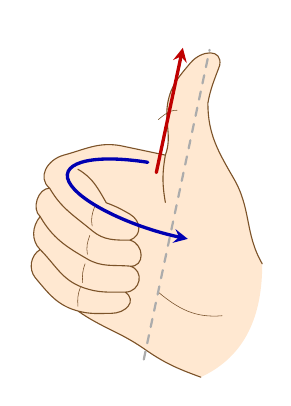
\begin{tikzpicture}[scale=.6,every node/.style={font=\small},>=stealth,
 line join=round,line cap=round]
\fill[orange!18] (2.9,-1.1)--(.85,1.2)--(-1.3,1.2)--(-1,-2.1)
--(.4,-2.9)--(1.6,-3.5) to[out=25,in=-90] cycle;
\draw[fill=orange!18,draw=brown!65!black] (2.9,-1.1) to[out=120,in=-60] (2.3,.7) to[out=120,in=-90]
(1.75,2.3) to[out=80,in=-110] (2,3.1)
to[out=80,in=50,looseness=1.5] (1.38,3.15)
to[out=-130,in=80] (.9,2.3) to[out=-100,in=70] (.85,1.2)
to[out=-100,in=100] (.85,.2)
(.85,1.2)--(-.1,1.4) to[out=170,in=15] (-1.3,1.2)
to[out=-165,in=140,looseness=1.2] (-1.6,.5)
to[out=-60,in=140] (-.7,-.4) to[out=-40,in=180] (.1,-.6)
to[out=20,in=-30,looseness=1.3] (.1,-.05)
to[out=150,in=-20] (-.4,.19) to[out=120,in=-30] (-1,.9)
(-1.6,.5) to[out=180,in=140] (-1.8,-.1)
to[out=-60,in=150] (-.8,-1) to[out=-30,in=175] (.1,-1.15)
to[out=-5,in=-15,looseness=1.5] (.1,-.6)
(-1.8,-.1) to[out=-130,in=135] (-1.8,-.8)
to[out=-45,in=160] (-.9,-1.6) to[out=-20,in=180] (0,-1.7)
to[out=0,in=-15,looseness=1.5] (.1,-1.15)
(-1.8,-.8) to[out=-150,in=130] (-1.9,-1.4)
to[out=-50,in=165] (-1,-2.1) to[out=-15,in=180] (-.3,-2.15)
to[out=0,in=-35,looseness=1.5] (0,-1.7)
(-1,-2.1) to[out=-35,in=145] (.4,-2.9) to[out=-35,in=160] (1.6,-3.5);
\draw[brown!60!black,very thin] (-.7,-.3) to[out=100,in=-110] (-.65,.1)
(-.8,-.9) to[out=100,in=-110] (-.75,-.5)
(-.9,-1.5) to[out=95,in=-110] (-.85,-1.1)
(-1,-2) to[out=95,in=-110] (-.95,-1.6)
(.7,1.95) to[out=40,in=180] (1.1,2.15)
(2.05,-2.2) to[out=-175,in=-40] (.7,-1.7);
\coordinate (O) at (1.1,.2);
\draw[gray!65,dashed,thick] (O)++(-102:3.4)--++(78:6.7);
\draw[->,red!75!black,very thick] (O)++(125:.77)--++(78:2.7)
 node[above] {$\manoNormal$};
\draw[->,blue!70!black,very thick,rotate=-15]
 (O)++(110:2.4 and .7) arc(110:280:2.4 and .7)
 node[below right] {$\manoRecorrido$};
\end{tikzpicture}
